% Created by tikzDevice version 0.10.1 on 2016-08-08 10:49:00
% !TEX encoding = UTF-8 Unicode
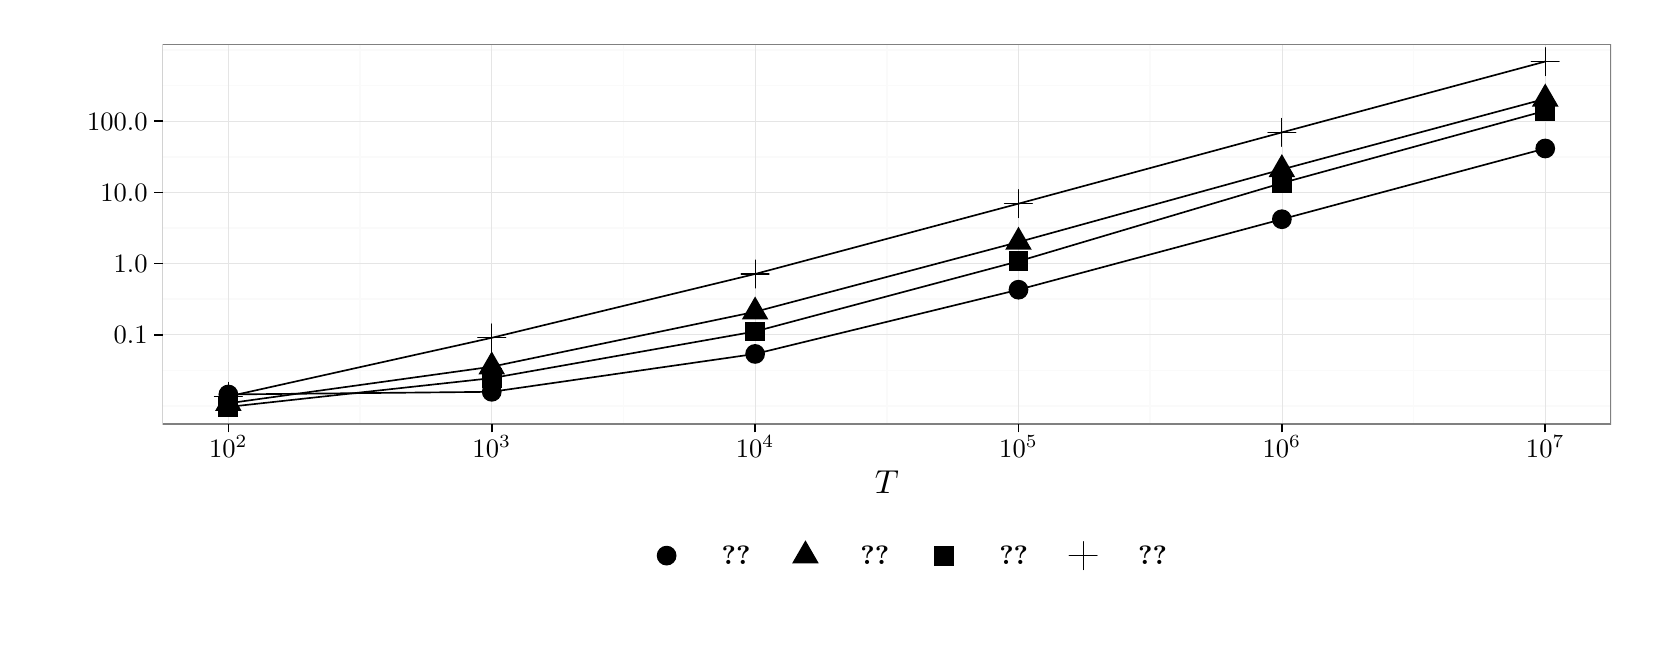
\begin{tikzpicture}[x=1pt,y=1pt]
\definecolor{fillColor}{RGB}{255,255,255}
\path[use as bounding box,fill=fillColor,fill opacity=0.00] (0,0) rectangle (578.16,216.81);
\begin{scope}
\path[clip] (  0.00,  0.00) rectangle (578.16,216.81);
\definecolor{drawColor}{RGB}{255,255,255}
\definecolor{fillColor}{RGB}{255,255,255}

\path[draw=drawColor,line width= 0.6pt,line join=round,line cap=round,fill=fillColor] (  0.00,  0.00) rectangle (578.16,216.81);
\end{scope}
\begin{scope}
\path[clip] ( 48.73, 73.54) rectangle (572.16,210.81);
\definecolor{fillColor}{RGB}{255,255,255}

\path[fill=fillColor] ( 48.73, 73.54) rectangle (572.16,210.81);
\definecolor{drawColor}{gray}{0.98}

\path[draw=drawColor,line width= 0.6pt,line join=round] ( 48.73, 80.12) --
	(572.16, 80.12);

\path[draw=drawColor,line width= 0.6pt,line join=round] ( 48.73, 92.98) --
	(572.16, 92.98);

\path[draw=drawColor,line width= 0.6pt,line join=round] ( 48.73,118.70) --
	(572.16,118.70);

\path[draw=drawColor,line width= 0.6pt,line join=round] ( 48.73,144.42) --
	(572.16,144.42);

\path[draw=drawColor,line width= 0.6pt,line join=round] ( 48.73,170.14) --
	(572.16,170.14);

\path[draw=drawColor,line width= 0.6pt,line join=round] ( 48.73,195.86) --
	(572.16,195.86);

\path[draw=drawColor,line width= 0.6pt,line join=round] ( 48.73,208.72) --
	(572.16,208.72);

\path[draw=drawColor,line width= 0.6pt,line join=round] (120.10, 73.54) --
	(120.10,210.81);

\path[draw=drawColor,line width= 0.6pt,line join=round] (215.27, 73.54) --
	(215.27,210.81);

\path[draw=drawColor,line width= 0.6pt,line join=round] (310.44, 73.54) --
	(310.44,210.81);

\path[draw=drawColor,line width= 0.6pt,line join=round] (405.61, 73.54) --
	(405.61,210.81);

\path[draw=drawColor,line width= 0.6pt,line join=round] (500.78, 73.54) --
	(500.78,210.81);
\definecolor{drawColor}{gray}{0.90}

\path[draw=drawColor,line width= 0.2pt,line join=round] ( 48.73,105.84) --
	(572.16,105.84);

\path[draw=drawColor,line width= 0.2pt,line join=round] ( 48.73,131.56) --
	(572.16,131.56);

\path[draw=drawColor,line width= 0.2pt,line join=round] ( 48.73,157.28) --
	(572.16,157.28);

\path[draw=drawColor,line width= 0.2pt,line join=round] ( 48.73,183.00) --
	(572.16,183.00);

\path[draw=drawColor,line width= 0.2pt,line join=round] ( 72.52, 73.54) --
	( 72.52,210.81);

\path[draw=drawColor,line width= 0.2pt,line join=round] (167.69, 73.54) --
	(167.69,210.81);

\path[draw=drawColor,line width= 0.2pt,line join=round] (262.86, 73.54) --
	(262.86,210.81);

\path[draw=drawColor,line width= 0.2pt,line join=round] (358.03, 73.54) --
	(358.03,210.81);

\path[draw=drawColor,line width= 0.2pt,line join=round] (453.20, 73.54) --
	(453.20,210.81);

\path[draw=drawColor,line width= 0.2pt,line join=round] (548.37, 73.54) --
	(548.37,210.81);
\definecolor{fillColor}{RGB}{0,0,0}

\path[fill=fillColor] ( 72.52, 84.27) circle (  3.57);

\path[fill=fillColor] ( 72.52, 86.63) --
	( 77.32, 78.31) --
	( 67.71, 78.31) --
	cycle;

\path[fill=fillColor] ( 68.95, 76.21) --
	( 76.09, 76.21) --
	( 76.09, 83.35) --
	( 68.95, 83.35) --
	cycle;
\definecolor{drawColor}{RGB}{0,0,0}

\path[draw=drawColor,line width= 0.4pt,line join=round,line cap=round] ( 67.47, 83.55) -- ( 77.57, 83.55);

\path[draw=drawColor,line width= 0.4pt,line join=round,line cap=round] ( 72.52, 78.51) -- ( 72.52, 88.60);

\path[fill=fillColor] (167.69, 85.23) circle (  3.57);

\path[fill=fillColor] (167.69, 99.85) --
	(172.49, 91.53) --
	(162.88, 91.53) --
	cycle;

\path[fill=fillColor] (164.12, 86.60) --
	(171.26, 86.60) --
	(171.26, 93.74) --
	(164.12, 93.74) --
	cycle;

\path[draw=drawColor,line width= 0.4pt,line join=round,line cap=round] (162.64,104.74) -- (172.74,104.74);

\path[draw=drawColor,line width= 0.4pt,line join=round,line cap=round] (167.69, 99.69) -- (167.69,109.78);

\path[fill=fillColor] (262.86, 98.91) circle (  3.57);

\path[fill=fillColor] (262.86,119.69) --
	(267.66,111.36) --
	(258.05,111.36) --
	cycle;

\path[fill=fillColor] (259.29,103.47) --
	(266.43,103.47) --
	(266.43,110.60) --
	(259.29,110.60) --
	cycle;

\path[draw=drawColor,line width= 0.4pt,line join=round,line cap=round] (257.81,127.80) -- (267.90,127.80);

\path[draw=drawColor,line width= 0.4pt,line join=round,line cap=round] (262.86,122.75) -- (262.86,132.84);

\path[fill=fillColor] (358.03,122.12) circle (  3.57);

\path[fill=fillColor] (358.03,144.89) --
	(362.83,136.57) --
	(353.22,136.57) --
	cycle;

\path[fill=fillColor] (354.46,128.82) --
	(361.60,128.82) --
	(361.60,135.95) --
	(354.46,135.95) --
	cycle;

\path[draw=drawColor,line width= 0.4pt,line join=round,line cap=round] (352.98,153.21) -- (363.07,153.21);

\path[draw=drawColor,line width= 0.4pt,line join=round,line cap=round] (358.03,148.16) -- (358.03,158.25);

\path[fill=fillColor] (453.20,147.59) circle (  3.57);

\path[fill=fillColor] (453.20,171.13) --
	(458.00,162.81) --
	(448.39,162.81) --
	cycle;

\path[fill=fillColor] (449.63,157.08) --
	(456.77,157.08) --
	(456.77,164.22) --
	(449.63,164.22) --
	cycle;

\path[draw=drawColor,line width= 0.4pt,line join=round,line cap=round] (448.15,178.96) -- (458.24,178.96);

\path[draw=drawColor,line width= 0.4pt,line join=round,line cap=round] (453.20,173.92) -- (453.20,184.01);

\path[fill=fillColor] (548.37,173.15) circle (  3.57);

\path[fill=fillColor] (548.37,196.65) --
	(553.17,188.32) --
	(543.56,188.32) --
	cycle;

\path[fill=fillColor] (544.80,183.20) --
	(551.94,183.20) --
	(551.94,190.34) --
	(544.80,190.34) --
	cycle;

\path[draw=drawColor,line width= 0.4pt,line join=round,line cap=round] (543.32,204.57) -- (553.41,204.57);

\path[draw=drawColor,line width= 0.4pt,line join=round,line cap=round] (548.37,199.52) -- (548.37,209.62);

\path[draw=drawColor,line width= 0.6pt,line join=round] ( 72.52, 84.27) --
	(167.69, 85.23) --
	(262.86, 98.91) --
	(358.03,122.12) --
	(453.20,147.59) --
	(548.37,173.15);

\path[draw=drawColor,line width= 0.6pt,line join=round] ( 72.52, 81.08) --
	(167.69, 94.30) --
	(262.86,114.14) --
	(358.03,139.34) --
	(453.20,165.58) --
	(548.37,191.10);

\path[draw=drawColor,line width= 0.6pt,line join=round] ( 72.52, 79.78) --
	(167.69, 90.17) --
	(262.86,107.03) --
	(358.03,132.39) --
	(453.20,160.65) --
	(548.37,186.77);

\path[draw=drawColor,line width= 0.6pt,line join=round] ( 72.52, 83.55) --
	(167.69,104.74) --
	(262.86,127.80) --
	(358.03,153.21) --
	(453.20,178.96) --
	(548.37,204.57);
\definecolor{drawColor}{gray}{0.50}

\path[draw=drawColor,line width= 0.6pt,line join=round,line cap=round] ( 48.73, 73.54) rectangle (572.16,210.81);
\end{scope}
\begin{scope}
\path[clip] (  0.00,  0.00) rectangle (578.16,216.81);
\definecolor{drawColor}{RGB}{0,0,0}

\node[text=drawColor,anchor=base east,inner sep=0pt, outer sep=0pt, scale=  0.96] at ( 43.33,102.53) {0.1};

\node[text=drawColor,anchor=base east,inner sep=0pt, outer sep=0pt, scale=  0.96] at ( 43.33,128.25) {1.0};

\node[text=drawColor,anchor=base east,inner sep=0pt, outer sep=0pt, scale=  0.96] at ( 43.33,153.97) {10.0};

\node[text=drawColor,anchor=base east,inner sep=0pt, outer sep=0pt, scale=  0.96] at ( 43.33,179.70) {100.0};
\end{scope}
\begin{scope}
\path[clip] (  0.00,  0.00) rectangle (578.16,216.81);
\definecolor{drawColor}{RGB}{0,0,0}

\path[draw=drawColor,line width= 0.6pt,line join=round] ( 45.73,105.84) --
	( 48.73,105.84);

\path[draw=drawColor,line width= 0.6pt,line join=round] ( 45.73,131.56) --
	( 48.73,131.56);

\path[draw=drawColor,line width= 0.6pt,line join=round] ( 45.73,157.28) --
	( 48.73,157.28);

\path[draw=drawColor,line width= 0.6pt,line join=round] ( 45.73,183.00) --
	( 48.73,183.00);
\end{scope}
\begin{scope}
\path[clip] (  0.00,  0.00) rectangle (578.16,216.81);
\definecolor{drawColor}{RGB}{0,0,0}

\path[draw=drawColor,line width= 0.6pt,line join=round] ( 72.52, 70.54) --
	( 72.52, 73.54);

\path[draw=drawColor,line width= 0.6pt,line join=round] (167.69, 70.54) --
	(167.69, 73.54);

\path[draw=drawColor,line width= 0.6pt,line join=round] (262.86, 70.54) --
	(262.86, 73.54);

\path[draw=drawColor,line width= 0.6pt,line join=round] (358.03, 70.54) --
	(358.03, 73.54);

\path[draw=drawColor,line width= 0.6pt,line join=round] (453.20, 70.54) --
	(453.20, 73.54);

\path[draw=drawColor,line width= 0.6pt,line join=round] (548.37, 70.54) --
	(548.37, 73.54);
\end{scope}
\begin{scope}
\path[clip] (  0.00,  0.00) rectangle (578.16,216.81);
\definecolor{drawColor}{RGB}{0,0,0}

\node[text=drawColor,anchor=base,inner sep=0pt, outer sep=0pt, scale=  0.96] at ( 72.52, 61.53) {$10^{2}$};

\node[text=drawColor,anchor=base,inner sep=0pt, outer sep=0pt, scale=  0.96] at (167.69, 61.53) {$10^{3}$};

\node[text=drawColor,anchor=base,inner sep=0pt, outer sep=0pt, scale=  0.96] at (262.86, 61.53) {$10^{4}$};

\node[text=drawColor,anchor=base,inner sep=0pt, outer sep=0pt, scale=  0.96] at (358.03, 61.53) {$10^{5}$};

\node[text=drawColor,anchor=base,inner sep=0pt, outer sep=0pt, scale=  0.96] at (453.20, 61.53) {$10^{6}$};

\node[text=drawColor,anchor=base,inner sep=0pt, outer sep=0pt, scale=  0.96] at (548.37, 61.53) {$10^{7}$};
\end{scope}
\begin{scope}
\path[clip] (  0.00,  0.00) rectangle (578.16,216.81);
\definecolor{drawColor}{RGB}{0,0,0}

\node[text=drawColor,anchor=base,inner sep=0pt, outer sep=0pt, scale=  1.20] at (310.44, 48.46) {$T$};
\end{scope}
\begin{scope}
\path[clip] (  0.00,  0.00) rectangle (578.16,216.81);
\definecolor{fillColor}{RGB}{255,255,255}

\path[fill=fillColor] (204.93, 14.54) rectangle (415.96, 37.53);
\end{scope}
\begin{scope}
\path[clip] (  0.00,  0.00) rectangle (578.16,216.81);
\definecolor{fillColor}{RGB}{255,255,255}

\path[fill=fillColor] (212.81, 18.80) rectangle (248.94, 33.26);
\end{scope}
\begin{scope}
\path[clip] (  0.00,  0.00) rectangle (578.16,216.81);
\definecolor{fillColor}{RGB}{0,0,0}

\path[fill=fillColor] (230.88, 26.03) circle (  3.57);
\end{scope}
\begin{scope}
\path[clip] (  0.00,  0.00) rectangle (578.16,216.81);
\definecolor{fillColor}{RGB}{255,255,255}

\path[fill=fillColor] (262.98, 18.80) rectangle (299.12, 33.26);
\end{scope}
\begin{scope}
\path[clip] (  0.00,  0.00) rectangle (578.16,216.81);
\definecolor{fillColor}{RGB}{0,0,0}

\path[fill=fillColor] (281.05, 31.58) --
	(285.85, 23.26) --
	(276.24, 23.26) --
	cycle;
\end{scope}
\begin{scope}
\path[clip] (  0.00,  0.00) rectangle (578.16,216.81);
\definecolor{fillColor}{RGB}{255,255,255}

\path[fill=fillColor] (313.15, 18.80) rectangle (349.29, 33.26);
\end{scope}
\begin{scope}
\path[clip] (  0.00,  0.00) rectangle (578.16,216.81);
\definecolor{fillColor}{RGB}{0,0,0}

\path[fill=fillColor] (327.65, 22.46) --
	(334.79, 22.46) --
	(334.79, 29.60) --
	(327.65, 29.60) --
	cycle;
\end{scope}
\begin{scope}
\path[clip] (  0.00,  0.00) rectangle (578.16,216.81);
\definecolor{fillColor}{RGB}{255,255,255}

\path[fill=fillColor] (363.33, 18.80) rectangle (399.46, 33.26);
\end{scope}
\begin{scope}
\path[clip] (  0.00,  0.00) rectangle (578.16,216.81);
\definecolor{drawColor}{RGB}{0,0,0}

\path[draw=drawColor,line width= 0.4pt,line join=round,line cap=round] (376.35, 26.03) -- (386.44, 26.03);

\path[draw=drawColor,line width= 0.4pt,line join=round,line cap=round] (381.39, 20.98) -- (381.39, 31.08);
\end{scope}
\begin{scope}
\path[clip] (  0.00,  0.00) rectangle (578.16,216.81);
\definecolor{drawColor}{RGB}{0,0,0}

\node[text=drawColor,anchor=base east,inner sep=0pt, outer sep=0pt, scale=  0.96] at (261.17, 22.72) {\ref{Scen:change_in_mean}};
\end{scope}
\begin{scope}
\path[clip] (  0.00,  0.00) rectangle (578.16,216.81);
\definecolor{drawColor}{RGB}{0,0,0}

\node[text=drawColor,anchor=base east,inner sep=0pt, outer sep=0pt, scale=  0.96] at (311.35, 22.72) {\ref{Scen:change_in_slope}};
\end{scope}
\begin{scope}
\path[clip] (  0.00,  0.00) rectangle (578.16,216.81);
\definecolor{drawColor}{RGB}{0,0,0}

\node[text=drawColor,anchor=base east,inner sep=0pt, outer sep=0pt, scale=  0.96] at (361.52, 22.72) {\ref{Scen:change_in_mean_and_slope}};
\end{scope}
\begin{scope}
\path[clip] (  0.00,  0.00) rectangle (578.16,216.81);
\definecolor{drawColor}{RGB}{0,0,0}

\node[text=drawColor,anchor=base east,inner sep=0pt, outer sep=0pt, scale=  0.96] at (411.69, 22.72) {\ref{Scen:change_in_mean_and_variance}};
\end{scope}
\end{tikzpicture}
